% !TEX root = dissertationmain.tex
%Chapter
\chapter{Methodology}
\label{chap:chapter1}
%Brief
\paragraph{}This chapter contains an in-depth analysis of the design and implementation stages carried out during this project. Initially, the design and goals of the application will be enumerated. Subsequently an analysis of the application’s infrastructure will be presented followed by an in-depth detail of the modules and submodules within the application’s programming. A test case scenario will be defined and executed to provide a proof of concept. The efficiency and accuracy among other factors based on the test scenario will be analysed during the discussion chapter of this thesis. 

%Section
\section{Design}
\label{sec:section1}

\paragraph{}The application design’s primary goal was to be able to detect vulnerable machines on a large-scale network infrastructure regardless of topology or host types by using machine learning techniques and automated tool outputs. However, there are several requirements the application must adhere to for it to be a viable tool during a security assessment. The application created for this thesis was done so strictly on a proof of concept bases.

The application was designed with the following requirements in mind:

\paragraph{}\textbf{Text progress output with multiple verbosity settings} allowing for an experienced tester to understand what the application is doing at any point in time during execution. This is critical as tools used during an assessment on live networks must not hinder or damage the network or its hosts in any way as to disrupt an organisations business.

\paragraph{}\textbf{Several input type parameters} for which the tester can utilise based on the current information known about the network. Such as only using one type of scan file and manually selecting the clustering model. 

\paragraph{}\textbf{Several output options including visually in the form of graphs} and to a dot type file to be used with other industry applications and reports.
\paragraph{}\textbf{Manual overriding of variables via parameters} in order to allow for the application to be scripted and modified by the tester. This will increase the efficiency of using the tool and provide advanced customisation of the algorithms within the application.

\paragraph{}\textbf{Highly versatile with working conditions and configurability.} The programming of the application to be highly documented allowing a tester to fix and modify the application code to suit the operation’s needs. By using a primarily interpreted language as appose to compiled one would allow for this, as well as making the application portable without extra code. For these purposes, the Python programming language was chosen. With the majority of modern tools and scripts used by penetration testers haven been written in Python due to its versatility, reliability and portability, it further enforces this choice.

\subsection{Application Brief}

\paragraph{}The application requires several parameters to run and has three different global modes; manual, assisted and automatic. These modes can either be run with Nmap, Nessus or both inputs with the majority of the use case scenarios requiring both. The application will then parse these inputs, process the data in several ways and cluster the information based on feature similarities. Output includes the full details of each cluster within the clustering. If using both inputs the application will combine the data from each and subtract large similarity clusters. By doing this, the application will determine the most unique hosts within the topology and display them in a new clustering. The unique hosts will, based on probability, be the most vulnerable on the network and should be prioritised by a tester during the manual assessment. This is due to the model prioritising the vulnerabilities each scanner detects then appends them to the pre-existing host set, thus rendering that host more unique than the others.

The difference between modes and parameters will be explained within the infrastructure analyses.


%Section
\section{Infrastructure}
\label{sec:section2}

%TODO notes
\begin{itemize}
\item Link to figure
\item Modes and parameters. Usage examples.
\item Explain nmap cluster library from blackhat and others.
\item Explain infrastructure.
\item followed by an in-depth detail of the modules and submodules within the application’s programming.
\item Explain cluster subclass.

\item Distance matrix and covariance coefficient matrix
\item provide a description of the mathematical concepts used such as
\item Gap statistic- http://web.stanford.edu/~hastie/Papers/gap.pdf
\item The elbow method
\item Create a Mathematical Model
\end{itemize}



%Section
\section{Proof of Concept Testing}
\label{sec:section4}


\begin{figure}
\centering
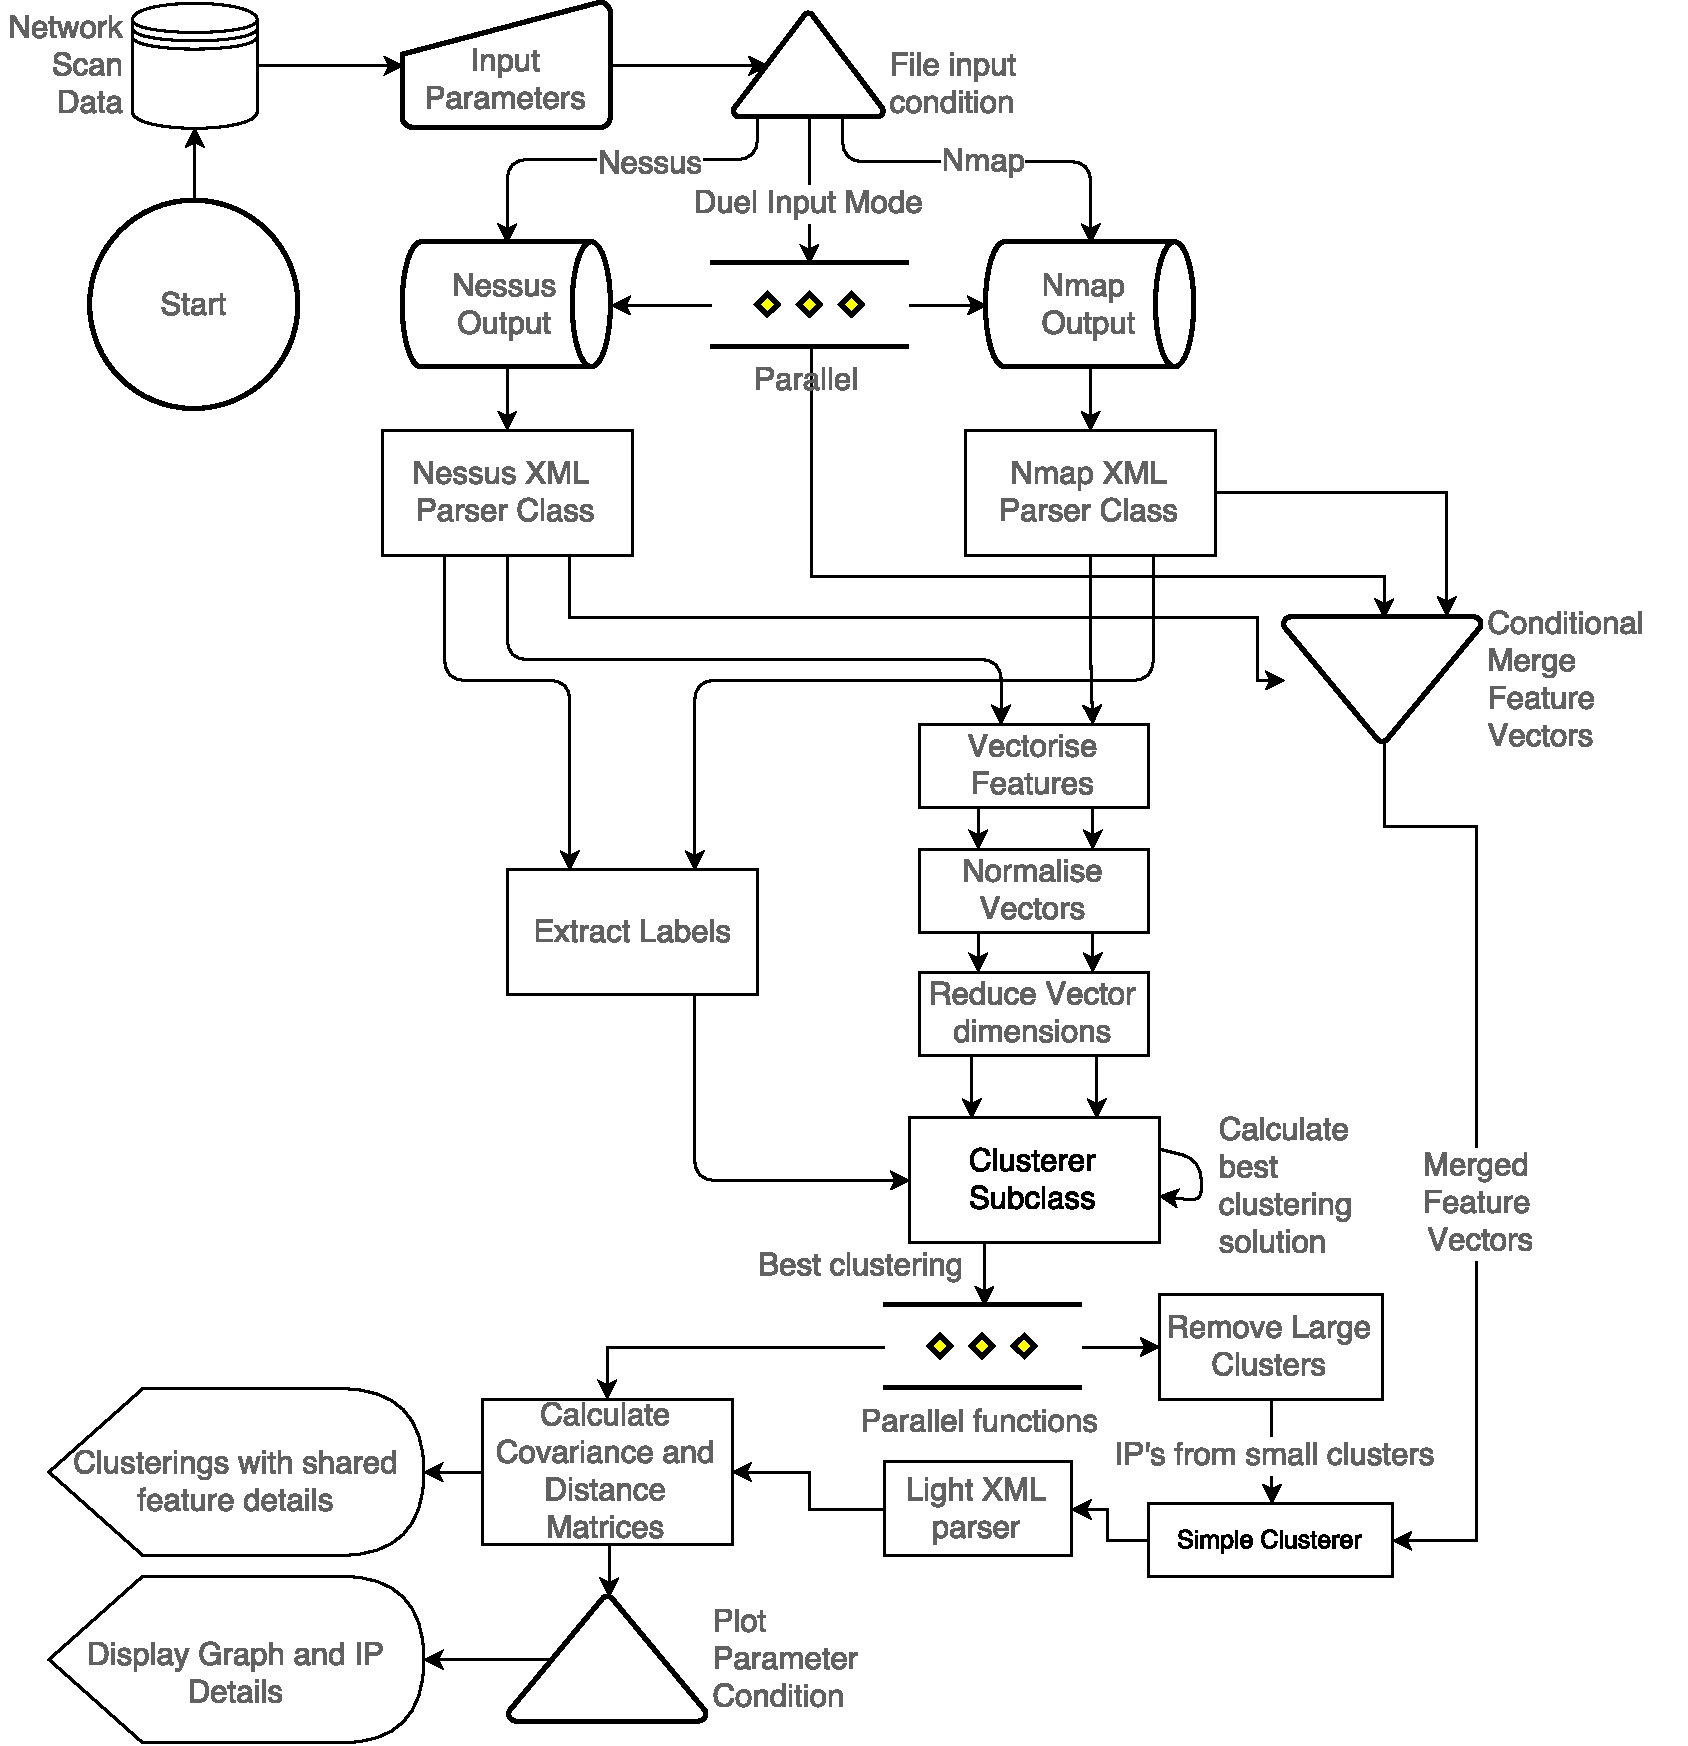
\includegraphics[width=4.5in]{./Figures/flow.pdf}
\caption{Application Infrastructure flow Diagram}
\label{flow}
\end{figure}